\documentclass[border=10pt]{standalone}
\usepackage{tikz}
\usetikzlibrary{arrows.meta,decorations.markings,calc}
\usepackage{amsmath}

\begin{document}
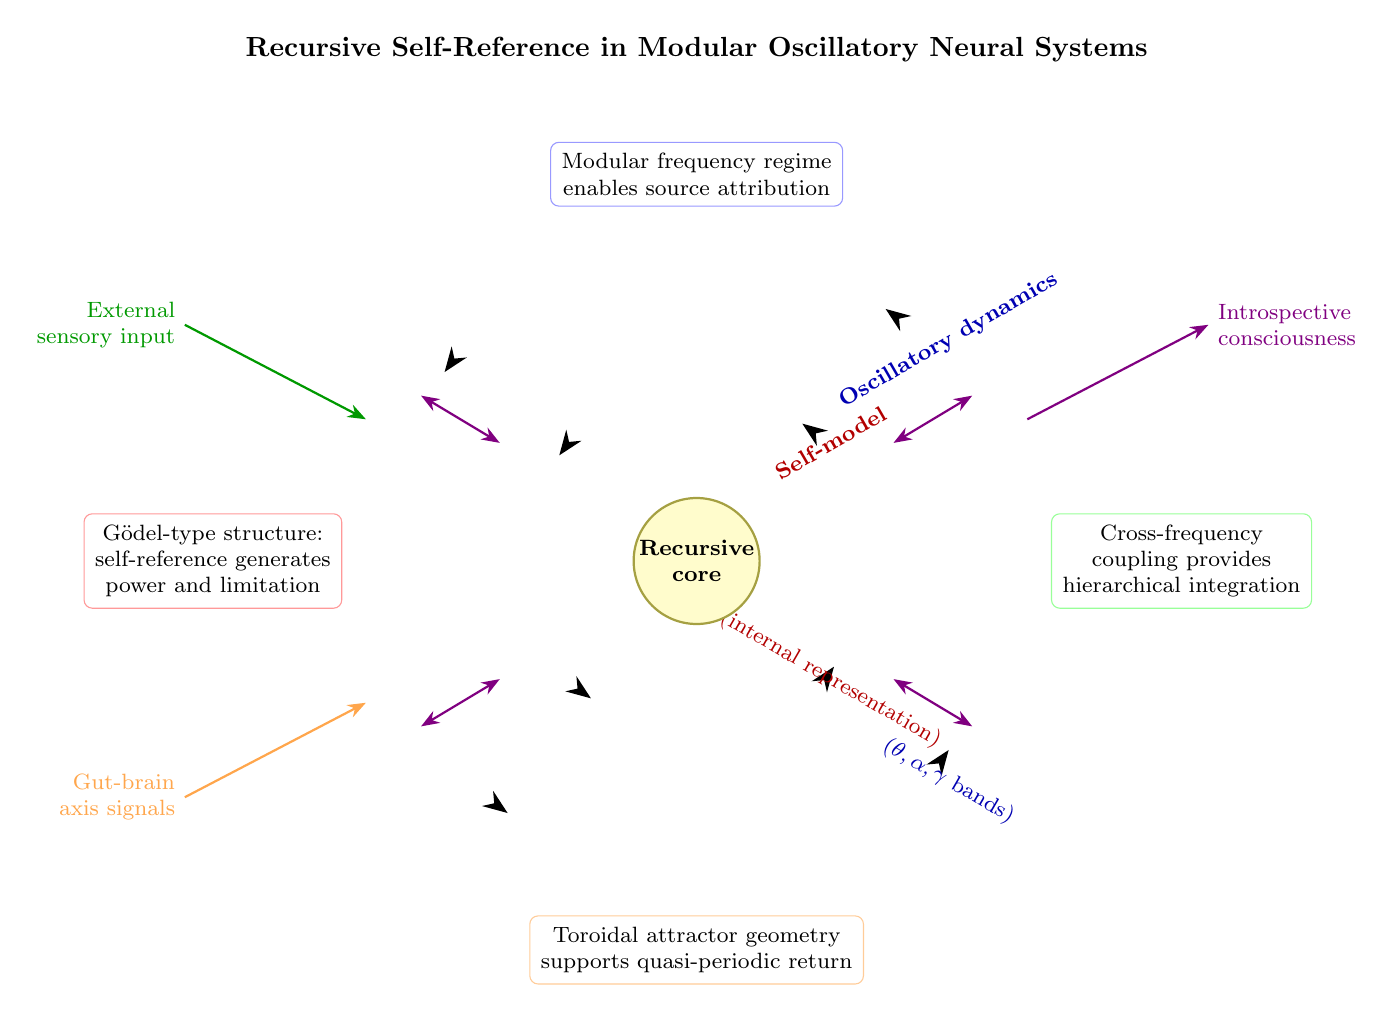
\begin{tikzpicture}[>=Stealth, font=\small]

% Outer loop: Neural oscillatory dynamics
\draw[very thick, blue!60, decorate, decoration={markings, 
  mark=at position 0.15 with {\arrow[scale=1.5]{>}},
  mark=at position 0.4 with {\arrow[scale=1.5]{>}},
  mark=at position 0.65 with {\arrow[scale=1.5]{>}},
  mark=at position 0.9 with {\arrow[scale=1.5]{>}}}] 
  (0,0) circle (4);
\node[font=\footnotesize\bfseries, blue!70!black, rotate=30] at (3.2,2.8) {Oscillatory dynamics};
\node[font=\footnotesize, blue!70!black, rotate=-30] at (3.2,-2.8) {($\theta, \alpha, \gamma$ bands)};

% Inner loop: Self-model / representation of own states
\draw[very thick, red!60, decorate, decoration={markings, 
  mark=at position 0.15 with {\arrow[scale=1.5]{>}},
  mark=at position 0.4 with {\arrow[scale=1.5]{>}},
  mark=at position 0.65 with {\arrow[scale=1.5]{>}},
  mark=at position 0.9 with {\arrow[scale=1.5]{>}}}] 
  (0,0) circle (2.2);
\node[font=\footnotesize\bfseries, red!70!black, rotate=30] at (1.7,1.5) {Self-model};
\node[font=\footnotesize, red!70!black, rotate=-30] at (1.7,-1.5) {(internal representation)};

% Center: recursive core
\fill[yellow!20, draw=yellow!60!black, thick] (0,0) circle (0.8);
\node[font=\footnotesize\bfseries, align=center] at (0,0) {Recursive\\core};

% Bidirectional arrows between loops
\draw[<->, thick, violet] (2.5,1.5) -- (3.5,2.1);
\draw[<->, thick, violet] (-2.5,-1.5) -- (-3.5,-2.1);
\draw[<->, thick, violet] (2.5,-1.5) -- (3.5,-2.1);
\draw[<->, thick, violet] (-2.5,1.5) -- (-3.5,2.1);

% Labels around the outside
% Top: Modular frequency regime
\node[above, font=\footnotesize, align=center, fill=white, draw=blue!40, rounded corners=3pt, inner sep=4pt] at (0,4.5) {Modular frequency regime\\enables source attribution};

% Right: Cross-frequency coupling
\node[right, font=\footnotesize, align=center, fill=white, draw=green!40, rounded corners=3pt, inner sep=4pt] at (4.5,0) {Cross-frequency\\coupling provides\\hierarchical integration};

% Bottom: Toroidal attractor
\node[below, font=\footnotesize, align=center, fill=white, draw=orange!40, rounded corners=3pt, inner sep=4pt] at (0,-4.5) {Toroidal attractor geometry\\supports quasi-periodic return};

% Left: Godel analogy
\node[left, font=\footnotesize, align=center, fill=white, draw=red!40, rounded corners=3pt, inner sep=4pt] at (-4.5,0) {G\"odel-type structure:\\self-reference generates\\power and limitation};

% External inputs
\draw[->, thick, green!60!black] (-6.5,3) -- (-4.2,1.8);
\node[left, font=\footnotesize, green!60!black, align=right] at (-6.5,3) {External\\sensory input};

\draw[->, thick, orange!70] (-6.5,-3) -- (-4.2,-1.8);
\node[left, font=\footnotesize, orange!70, align=right] at (-6.5,-3) {Gut-brain\\axis signals};

% Output
\draw[->, thick, violet] (4.2,1.8) -- (6.5,3);
\node[right, font=\footnotesize, violet, align=left] at (6.5,3) {Introspective\\consciousness};

% Title
\node[font=\normalsize\bfseries] at (0,6.5) {Recursive Self-Reference in Modular Oscillatory Neural Systems};

\end{tikzpicture}
\end{document}
